\documentclass[a4paper,12pt]{article} % добавить leqno в [] для нумерации слева

\usepackage{lab_preamble}

\begin{document}

\LabTitle{number}{text}

\tableofcontents

\textbf{Цель работы}:
\begin{enumerate}
  \item исследовать явление акустического резонанса в тонком стержне.
  \item измерить скорость распространения продольных звуковых колебаний в тонких стержнях из различных материалов и различных размеров.
  \item измерить модули Юнга различных материалов.
\end{enumerate}

\textbf{Приборы}:
\begin{enumerate}
  \item генератор звуковых частот
  \item частотомер
  \item осциллограф
  \item электромагнитные излучатель и приёмник колебаний
  \item набор стержней из различных материалов
\end{enumerate}

\section{Краткая Теория.}
\subsection{Введение.}
Закон гука:
\begin{equation}
  \sigma =  \varepsilon E
  \label{eq:1}
\end{equation}

Малые деформации твердых тел вызывают волны, которые называют акустическими или звуковыми.
Волны сжатия/растяжения, распространяющиеся вдоль оси, по которой происходит деформация, называются продольными.

\begin{equation}
  u =  \sqrt{\frac{E}{\rho}}
  \label{eq:2}
\end{equation}
, где u - скорость распространения продольной акустической волны, 
$\rho$ - плотность среды.

Характерные значения модуля Юнга металлов лежат в диапазоне $E \sim (10^{10} - 10^{12}) \text{Па}$, так как при плотности $\rho \sim 10^4 \text{кг}/\text{м}^3$ характерные значения скорости звука в
твёрдых телах составляют $u \sim (10^3 - 10^4) \text{м/с}$.

Рассмотрим стержень постоянного круглого сечения, радиус R которого много меньше его длины L. С точки зрения распространения волн стержень можно считать тонким, если длина $\lambda$ звуковых волн в нём велика по сравнению с его радиусом: $\lambda \gg R$.

\subsection{Уравнение волны в тонком стержне}
Пусть плоскость среды, находящаяся исходно в точке x,
сместилась к моменту t на расстояние $\xi(x,t)$.

\begin{equation}
  \varepsilon = \partderiv{\xi}{x}
  \label{eq:3}
\end{equation}

\eqref{eq:1} implies

\begin{equation}
  \sigma =  \varepsilon E = E \partderiv{\xi}{x}
  \label{eq:4}
\end{equation}

\begin{figure} [h] \center
  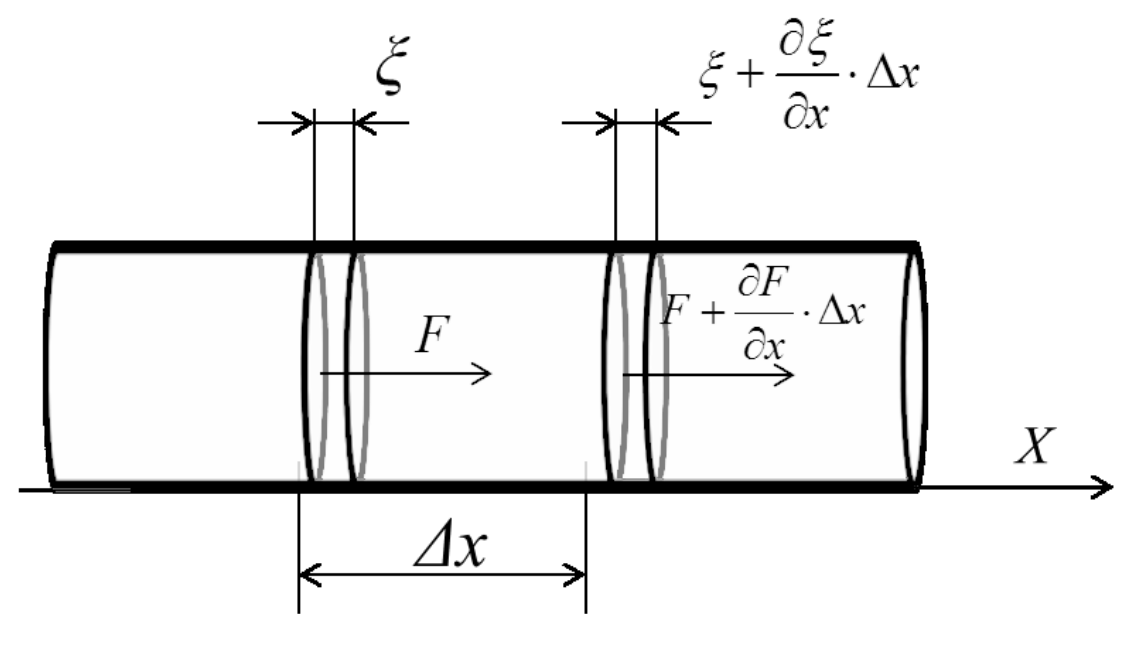
\includegraphics[scale=0.3]{148/pic 1.png}
  \caption[Рис. 1]{Силы, действующие на элемент стержня при продольных колебаниях}
\end{figure}

\begin{equation}
  \Delta F = S \D{x} \partderiv{\sigma}{x} = 
  \partderiv[2]{\xi}{x} E S \D{x}
  \label{eq:5}
\end{equation}

Волновое уравнение:
\begin{equation}
  \partderiv[2]{\xi}{t} = u^2 \partderiv[2]{\xi}{x}
  \label{eq:6}
\end{equation}

При $\lambda \ll R$:
\[ u_i = \sqrt{\frac{E}{\rho} \cdot \frac{1-\mu}{(1+\mu)(1-2\mu)}} \]
\label{eq:ui}

\subsection{Бегущие акустические волны. Скорость волны}
Общее решение волнового ур-ия \eqref{eq:6}:
\begin{equation}
  \xi(x,t) = \phi_1(x-ut) + \phi_2(x+ut)
  \label{eq:7}
\end{equation}

\subsection{Собственные колебания стержня. Стоячие волны}
В случае гармонического возбуждения:
\begin{equation}
  \xi(x,t) = A_1 \sin{(\omega t - kx + \varphi_1)} + 
  A_2 \sin{(\omega t + kx + \varphi_2)}
  \label{eq:8}
\end{equation}
$\omega = 2\pi f$ - циклическая частота, 
$k = \frac{2\pi}{\lambda}$ - волновое число или пространственная частота волны.

Если конци не закреплены:
\begin{equation}
  \sigma(0) = 0 \implies \partderiv{\xi}{x} (x = 0) = 0,\ 
  \sigma(L) = 0 \implies \partderiv{\xi}{x} (x = L) = 0
  \label{eq:9}
\end{equation}

\eqref{eq:8} и \eqref{eq:9} $\implies$
\begin{equation}
  A_1 = A_2 \label{eq:10}
\end{equation}
\begin{equation}
  \varphi_1 = \varphi_2 \label{eq:10}
\end{equation}

\section{Выполнение.} \label{Выполнение}
\begin{enumerate}
  \item \label{Выполнение:1}
  \item \label{Выполнение:2}
  \item \label{Выполнение:3}
  \item \label{Выполнение:4}
  \item \label{Выполнение:5}
  \item \label{Выполнение:6}
  \item \label{Выполнение:7}
  \item \label{Выполнение:8}
  \item \label{Выполнение:9}
  \item \label{Выполнение:10}
  \item \label{Выполнение:11}
  \item \label{Выполнение:12}
\end{enumerate}

\section{Вывод}

\end{document}